\documentclass{article}
\usepackage{amsmath}
\usepackage{amsfonts}
\usepackage{geometry}
\usepackage{booktabs}
\usepackage{tcolorbox}
\usepackage{tikz}
\usetikzlibrary{arrows.meta, patterns}

\geometry{a4paper, margin=1in}

\begin{document}

\title{Statics}
\author{}
\date{}
\maketitle


\section{Fundamental Forces (Big Picture)}
In nature, all interactions in the universe can be reduced to four fundamental forces. In high-school mechanics, we only deal with the first two, but it is important to understand the big picture:
\begin{itemize}
  \item \textbf{Gravitational Force:} An attractive force between any two objects with mass. It has an infinite range but is by far the \emph{weakest} of the four forces. In mechanics, this is responsible for an object's weight ($\vec{F}_g = m\vec{g}$).
  \item \textbf{Electromagnetic Force:} A force between charged particles. Like gravity, it has an infinite range, but it is much stronger. \textbf{Crucially}, this force is responsible for almost all \emph{everyday push/pull contact forces}. When you push a wall, the electrons in your hand repel the electrons in the wall—this is the origin of the Normal Force, Friction, Tension, and Spring forces!
  \item \textbf{Strong Nuclear Force:} A very short-range force that binds protons and neutrons together inside the nucleus of an atom. It is the strongest force in nature, but its range is limited to the subatomic level.
  \item \textbf{Weak Nuclear Force:} Another short-range force responsible for certain types of radioactive decay (like beta decay) and nuclear fusion in the sun. 
\end{itemize}
Because dealing with molecular repulsion and quantum mechanics is too complex for studying macroscopic motion, we \emph{categorize} the macroscopic effects of the electromagnetic force into simplified models. For problem-solving, you typically do \emph{not} write these four fundamental forces directly; instead, you use the ``Common Forces'' listed below.
\subsection{Common Forces}
In most mechanics problems, you will see the same few forces again and again. The key skill is to \textbf{identify which forces actually act} on the chosen object, then decide their directions before writing any equations.

\begin{table}[h]
 \centering
 \caption{Common Forces in High-School Mechanics}
 \begin{tabular}{lll}
   \toprule
   \textbf{Force} & \textbf{Symbol} & \textbf{Typical Direction / Notes} \\ \midrule
   Weight (gravity) & $\vec{W}=m\vec{g}$ & Downward \\
   Normal force & $\vec{N}$ & Perpendicular to a surface \\
   Tension & $\vec{T}$ & Along a rope/string (ideal: same in one rope segment) \\
   Friction (static/kinetic) & $\vec{f}_s,\ \vec{f}_k$ & Along a surface, opposes (relative) motion \\
   \bottomrule
 \end{tabular}
\end{table}

\newpage

\section{Weight and Gravitational Field Strength}


% --- 图 1: 静止在水平面上的物体 (Basic Weight) ---
\begin{figure}[h]
    \centering
    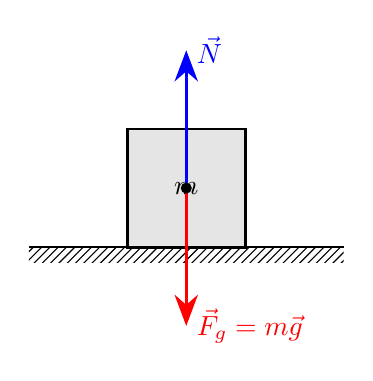
\begin{tikzpicture}[line width=1pt]
        % 地面
        \draw[thick] (-2,0) -- (2,0);
        \fill[pattern=north east lines] (-2,-0.2) rectangle (2,0);
        
        % 物体
        \draw[fill=gray!20] (-0.75,0) rectangle (0.75,1.5);
        \node at (0, 0.75) {$m$};
        
        % 力的矢量 (FBD)
        \draw[-{Stealth[scale=1.5]}, red] (0, 0.75) -- (0, -1) node[right] {$\vec{F}_g = m\vec{g}$};
        \draw[-{Stealth[scale=1.5]}, blue] (0, 0.75) -- (0, 2.5) node[right] {$\vec{N}$};
        
        % 中心点
        \fill (0,0.75) circle (2pt);
    \end{tikzpicture}
    \caption{Free-Body Diagram of an object at rest on a surface.}
\end{figure}

\subsection{Definition of Weight ($\vec{F}_g$)}
In physics, \textbf{Weight} (also referred to as the \textbf{Force of Gravity}, $\vec{F}_g$) is the gravitational force exerted by a large body, such as Earth, on an object. Unlike \textbf{mass} ($m$), which is an intrinsic scalar property of an object, weight is a \textbf{vector quantity} that depends on the local gravitational environment.

\subsection{The Relationship: $\vec{F}_g = m\vec{g}$}
Near the surface of the Earth, the magnitude of the gravitational force is directly proportional to the mass of the object. This relationship is defined by:

\begin{equation}
\vec{F}_g = m\vec{g}
\end{equation}

Where:
\begin{itemize}
    \item $\vec{F}_g$ is the \textbf{force of gravity} (Weight), measured in Newtons ($\text{N}$).
    \item $m$ is the \textbf{mass} of the object, measured in kilograms ($\text{kg}$).
    \item $\vec{g}$ is the \textbf{gravitational field strength}. Near Earth's surface, $|\vec{g}| \approx 9.8\,\text{N/kg}$ (or $9.8\,\text{m/s}^2$).
\end{itemize}

\subsection{Newton's Law of Universal Gravitation}
While $\vec{F}_g = m\vec{g}$ is useful near the surface of a specific planet like Earth, Newton's Law of Universal Gravitation provides the fundamental equation for the gravitational force between \emph{any} two masses in the universe. It states that the gravitational force is directly proportional to the product of their masses and inversely proportional to the square of the distance between their centers.

\begin{equation}
F_g = G \frac{m_1 m_2}{r^2}
\end{equation}

\begin{figure}[h]
    \centering
    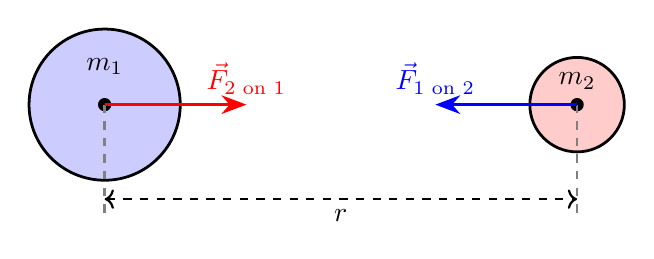
\begin{tikzpicture}[scale=1.2, line width=1pt]
        % Mass 1
        \draw[fill=blue!20] (0,0) circle (0.8);
        \node at (0, 0.4) {$m_1$};
        \fill (0,0) circle (2pt);
        
        % Mass 2
        \draw[fill=red!20] (5,0) circle (0.5);
        \node at (5, 0.25) {$m_2$};
        \fill (5,0) circle (2pt);
        
        % Distance r
        \draw[<->, dashed, thick] (0,-1.0) -- (5,-1.0) node[midway, below] {$r$};
        \draw[dashed, gray] (0,0) -- (0,-1.2);
        \draw[dashed, gray] (5,0) -- (5,-1.2);
        
        % Force vectors
        \draw[-{Stealth[scale=1.2]}, red] (0,0) -- (1.5,0) node[above] {$\vec{F}_{2 \text{ on } 1}$};
        \draw[-{Stealth[scale=1.2]}, blue] (5,0) -- (3.5,0) node[above] {$\vec{F}_{1 \text{ on } 2}$};
    \end{tikzpicture}
    \caption{Universal Gravitation: Two masses exert equal and opposite attractive forces on each other.}
\end{figure}

Where:
\begin{itemize}
    \item $F_g$ is the magnitude of the gravitational force between the two objects ($\text{N}$).
    \item $G$ is the \textbf{Universal Gravitational Constant} ($G \approx 6.67 \times 10^{-11}\,\text{N}\cdot\text{m}^2/\text{kg}^2$). This is a universal constant, unlike $g$ which changes depending on location.
    \item $m_1$ and $m_2$ are the masses of the two interacting objects ($\text{kg}$).
    \item $r$ is the distance between the \textbf{centers} of the two objects ($\text{m}$).
\end{itemize}

\subsubsection{Deriving Surface Gravity ($g$)}
By comparing the two equations for gravity for an object of mass $m$ on the surface of a planet (mass $M$, radius $r$), we can calculate the gravitational field strength $g$ of that planet:

\begin{equation}
mg = G \frac{Mm}{r^2} \implies g = \frac{GM}{r^2}
\end{equation}

\subsection{Key Concepts}
\begin{enumerate}
    \item \textbf{Direction:} The direction of the weight vector $\vec{F}_g$ is always directed \textbf{straight down} toward the center of the Earth, regardless of whether the object is moving upward, downward, or is at rest.
    \item \textbf{Field Strength Variations:} The value of $g$ is not a universal constant. It varies slightly with \textbf{latitude} (due to Earth's rotation and shape) and decreases with \textbf{altitude} (as the distance from Earth's center increases).
    \item \textbf{Mass vs. Weight:} 
    \begin{itemize}
        \item \textbf{Mass} is a measure of the amount of matter and inertia; it remains constant everywhere in the universe.
        \item \textbf{Weight} changes depending on the local value of $g$. For example, an astronaut's mass on the Moon is the same as on Earth, but their weight is approximately $1/6$ of its Earth value because $g_{\text{moon}} \approx 1.6\,\text{N/kg}$.
    \end{itemize}
\end{enumerate}

\newpage

\section{Common Contact Forces}

\subsection{Normal Force ($\vec{N}$)}
The normal force is a contact force from a surface, acting perpendicular (``normal'') to that surface. It represents the surface pushing back to prevent the object from falling through it. 

A common mistake is to always assume $\vec{N} = m\vec{g}$. The normal force is a \emph{reactive force}, it takes whatever value is needed to satisfy Newton's 2nd Law in the direction perpendicular to the surface.
\begin{itemize}
    \item \textbf{Level Ground (No other vertical forces):} $N = mg$
    \item \textbf{Level Ground (Pulling up slightly):} $N < mg$ (The ground doesn't need to push as hard).
    \item \textbf{Level Ground (Pushing down):} $N > mg$ (The ground must push harder to balance gravity plus your push).
    \item \textbf{Inclined Plane:} $N = mg\cos\theta$ (Assuming no acceleration perpendicular to the incline).
    \item \textbf{Vertical Wall:} If you push a book horizontally against a wall, the normal force from the wall equals your horizontal push, and is entirely unrelated to gravity!
\end{itemize}

\begin{figure}[h]
    \centering
    % Diagram 1: Level ground, N=mg
    \begin{minipage}{0.31\textwidth}
        \centering
        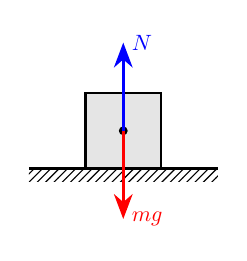
\begin{tikzpicture}[scale=0.8, transform shape, line width=1pt]
            \draw[thick] (-1.5,0) -- (1.5,0);
            \fill[pattern=north east lines] (-1.5,-0.2) rectangle (1.5,0);
            \draw[fill=gray!20] (-0.6,0) rectangle (0.6,1.2);
            \fill (0,0.6) circle (2pt);
            \draw[-{Stealth[scale=1.2]}, red] (0,0.6) -- (0,-0.8) node[right] {$mg$};
            \draw[-{Stealth[scale=1.2]}, blue] (0,0.6) -- (0,2) node[right] {$N$};
        \end{tikzpicture}
        
        \vspace{0.2cm}
        \small (a) $N = mg$
    \end{minipage}%
    \hfill
    % Diagram 2: Pulling up
    \begin{minipage}{0.31\textwidth}
        \centering
        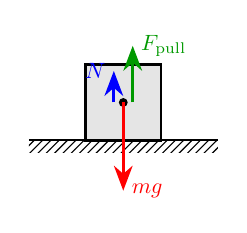
\begin{tikzpicture}[scale=0.8, transform shape, line width=1pt]
            \draw[thick] (-1.5,0) -- (1.5,0);
            \fill[pattern=north east lines] (-1.5,-0.2) rectangle (1.5,0);
            \draw[fill=gray!20] (-0.6,0) rectangle (0.6,1.2);
            \fill (0,0.6) circle (2pt);
            \draw[-{Stealth[scale=1.2]}, red] (0,0.6) -- (0,-0.8) node[right] {$mg$};
            \draw[-{Stealth[scale=1.2]}, green!60!black] (0.15,0.6) -- (0.15,1.5) node[right] {$F_{\text{pull}}$};
            \draw[-{Stealth[scale=1.2]}, blue] (-0.15,0.6) -- (-0.15,1.1) node[left] {$N$};
        \end{tikzpicture}
        
        \vspace{0.2cm}
        \small (b) Pulling up ($N < mg$)
    \end{minipage}%
    \hfill
    % Diagram 3: Pushing down
    \begin{minipage}{0.31\textwidth}
        \centering
        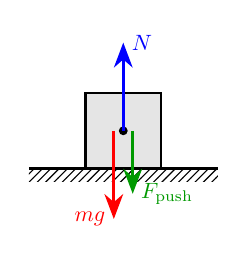
\begin{tikzpicture}[scale=0.8, transform shape, line width=1pt]
            \draw[thick] (-1.5,0) -- (1.5,0);
            \fill[pattern=north east lines] (-1.5,-0.2) rectangle (1.5,0);
            \draw[fill=gray!20] (-0.6,0) rectangle (0.6,1.2);
            \fill (0,0.6) circle (2pt);
            \draw[-{Stealth[scale=1.2]}, red] (-0.15,0.6) -- (-0.15,-0.8) node[left] {$mg$};
            \draw[-{Stealth[scale=1.2]}, green!60!black] (0.15,0.6) -- (0.15,-0.4) node[right] {$F_{\text{push}}$};
            \draw[-{Stealth[scale=1.2]}, blue] (0,0.6) -- (0,2) node[right] {$N$};
        \end{tikzpicture}
        
        \vspace{0.2cm}
        \small (c) Pushing down ($N > mg$)
    \end{minipage}

    \vspace{0.6cm}

    % Diagram 4: Incline
    \begin{minipage}{0.45\textwidth}
        \centering
        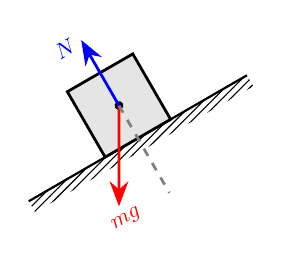
\begin{tikzpicture}[scale=0.8, transform shape, line width=1pt, rotate=30]
            \draw[thick] (-2,0) -- (2,0);
            \fill[pattern=north east lines] (-2,-0.2) rectangle (2,0);
            \draw[fill=gray!20] (-0.6,0) rectangle (0.6,1.2);
            \fill (0,0.6) circle (2pt);
            \draw[-{Stealth[scale=1.2]}, red] (0,0.6) -- ++(-120:1.6) node[below] {$mg$};
            \draw[dashed, gray] (0,0.6) -- ++(-90:1.6); % normal line
            \draw[-{Stealth[scale=1.2]}, blue] (0,0.6) -- (0,1.8) node[left] {$N$};
        \end{tikzpicture}
        
        \vspace{0.2cm}
        \small (d) Incline ($N = mg\cos\theta$)
    \end{minipage}%
    \hspace{0.05\textwidth}%
    % Diagram 5: Wall
    \begin{minipage}{0.45\textwidth}
        \centering
        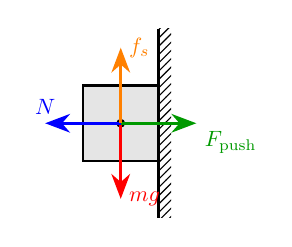
\begin{tikzpicture}[scale=0.8, transform shape, line width=1pt]
            \draw[thick] (0,-1.5) -- (0,1.5);
            \fill[pattern=north east lines] (0,-1.5) rectangle (0.2,1.5);
            \draw[fill=gray!20] (-1.2,-0.6) rectangle (0,0.6);
            \fill (-0.6,0) circle (2pt);
            \draw[-{Stealth[scale=1.2]}, red] (-0.6,0) -- (-0.6,-1.2) node[right] {$mg$};
            \draw[-{Stealth[scale=1.2]}, green!60!black] (-0.6,0) -- (0.6,0) node[below right] {$F_{\text{push}}$};
            \draw[-{Stealth[scale=1.2]}, blue] (-0.6,0) -- (-1.8,0) node[above] {$N$};
            \draw[-{Stealth[scale=1.2]}, orange] (-0.6,0) -- (-0.6,1.2) node[right] {$f_s$};
        \end{tikzpicture}
        
        \vspace{0.2cm}
        \small (e) Wall ($N = F_{\text{push}}$)
    \end{minipage}
    
    \caption{Free-Body Diagrams illustrating different Normal Force scenarios.}
\end{figure}

\subsection{Tension ($\vec{T}$)}
Tension is the pulling force transmitted along a rope, string, or cable. 
\begin{itemize}
    \item \textbf{Direction:} ``You can't push on a rope.'' Tension always acts \emph{along} the rope and pulls \emph{away} from the object it is attached to.
    \item \textbf{Action on different objects:} A rope pulls inward on both ends. Thus, the tension force at one end points in the opposite direction from the tension force at the other end.
    \item \textbf{Ideal Model Setup:} In high school physics, we typically assume ropes are \emph{massless} and pulleys are \emph{frictionless}. Under this ideal model, the tension $T$ has the same magnitude everywhere along one continuous segment of rope.
\end{itemize}

\begin{figure}[h]
    \centering
    % Diagram 1: Direction (Pulls away at an angle)
    \begin{minipage}{0.45\textwidth}
        \centering
        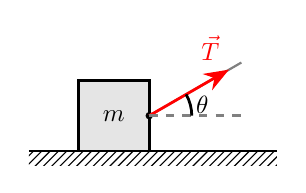
\begin{tikzpicture}[scale=0.9, transform shape, line width=1pt]
            % Ground
            \draw[thick] (-1.5,0) -- (2.0,0);
            \fill[pattern=north east lines] (-1.5,-0.2) rectangle (2.0,0);
            
            % Mass
            \draw[fill=gray!20] (-0.8,0) rectangle (0.2,1.0);
            \node at (-0.3, 0.5) {$m$};
            
            % Attach point
            \fill (0.2, 0.5) circle (1.5pt); 
            
            % Rope & force vector at an angle
            \draw[thick, gray] (0.2, 0.5) -- (1.5, 1.25); % rope
            \draw[-{Stealth[scale=1.2]}, red] (0.2, 0.5) -- ++(30:1.3) node[above left] {$\vec{T}$};
            
            % Dashed line for angle
            \draw[dashed, gray] (0.2, 0.5) -- (1.5, 0.5);
            
            % Angle arc
            \draw (0.8, 0.5) arc (0:30:0.6);
            \node at (0.95, 0.65) {$\theta$};
        \end{tikzpicture}
        
        \vspace{0.2cm}
        \small (a) Pulling at an angle
    \end{minipage}%
    \hfill
    % Diagram 2: Ideal Pulley
    \begin{minipage}{0.45\textwidth}
        \centering
        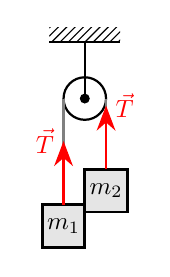
\begin{tikzpicture}[scale=0.9, transform shape, line width=1pt]
            % Pulley at origin
            \draw[thick, fill=white] (0,0) circle (0.3);
            \fill (0,0) circle (2pt);
            % Support
            \draw[thick] (0,0) -- (0,0.8);
            \draw[thick] (-0.5,0.8) -- (0.5,0.8);
            \fill[pattern=north east lines] (-0.5,0.8) rectangle (0.5,1.0);
            
            % Rope
            \draw[thick, gray] (-0.3,0) -- (-0.3,-1.5);
            \draw[thick, gray] (0.3,0) -- (0.3,-1.0);
            
            % Mass 1
            \draw[fill=gray!20] (-0.6,-2.1) rectangle (0,-1.5);
            \node at (-0.3,-1.8) {$m_1$};
            
            % Mass 2
            \draw[fill=gray!20] (0,-1.6) rectangle (0.6,-1.0);
            \node at (0.3,-1.3) {$m_2$};
            
            % Tensions
            \draw[-{Stealth[scale=1.2]}, red] (-0.3,-1.5) -- (-0.3,-0.6) node[left] {$\vec{T}$};
            \draw[-{Stealth[scale=1.2]}, red] (0.3,-1.0) -- (0.3,-0.1) node[right] {$\vec{T}$};
        \end{tikzpicture}
        
        \vspace{0.2cm}
        \small (b) Ideal pulley (magnitude $T$ is the same)
    \end{minipage}
    
    \caption{Free-Body Diagrams illustrating properties of Tension force.}
\end{figure}


\newpage

\section{Friction ($\vec{f}_s$ and $\vec{f}_k$)}
Friction is a contact force parallel to a surface that opposes relative motion (or the tendency to slip). It arises from the microscopic interaction between surfaces.

\subsection{Static Friction ($\vec{f}_s$)}
Static friction occurs when two surfaces are \textbf{not} slipping relative to each other. It helps keep an object at rest or prevents it from sliding.
\begin{itemize}
    \item \textbf{Variable Force:} Static friction is a "smart" force. It matches the applied opposing force perfectly, up until a breaking point.
    \item \textbf{Formula:} The value of static friction can be anything from zero up to a maximum value:
    \begin{equation}
        0 \le f_s \le f_{s,\text{max}} = \mu_s N
    \end{equation}
    where $\mu_s$ is the coefficient of static friction, and $N$ is the normal force.
    \item \textbf{Common Mistake:} DO NOT automatically set $f_s = \mu_s N$. That formula only gives you the \emph{maximum possible} static friction right before the object starts to slip.
\end{itemize}

\begin{figure}[h]
    \centering
    % Diagram 1: Small Push
    \begin{minipage}{0.45\textwidth}
        \centering
        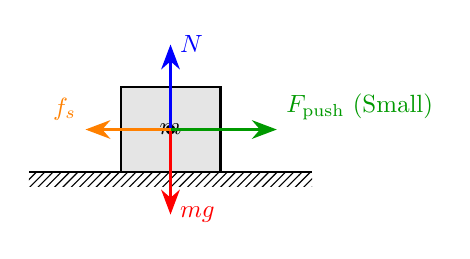
\begin{tikzpicture}[scale=0.9, transform shape, line width=1pt]
            % Ground
            \draw[thick] (-2,0) -- (2,0);
            \fill[pattern=north east lines] (-2,-0.2) rectangle (2,0);
            
            % Mass
            \draw[fill=gray!20] (-0.7,0) rectangle (0.7,1.2);
            \node at (0, 0.6) {$m$};
            \fill (0, 0.6) circle (2pt);
            
            % Forces
            \draw[-{Stealth[scale=1.2]}, red] (0, 0.6) -- (0, -0.6) node[right] {$mg$};
            \draw[-{Stealth[scale=1.2]}, blue] (0, 0.6) -- (0, 1.8) node[right] {$N$};
            
            % Small push and friction
            \draw[-{Stealth[scale=1.2]}, green!60!black] (0, 0.6) -- (1.5, 0.6) node[above right] {$F_{\text{push}}$ (Small)};
            \draw[-{Stealth[scale=1.2]}, orange] (0, 0.6) -- (-1.2, 0.6) node[above left] {$f_s$};
        \end{tikzpicture}
        
        \vspace{0.2cm}
        \small (a) Object at rest: $f_s = F_{\text{push}}$
    \end{minipage}%
    \hfill
    % Diagram 2: Incline (Max friction)
    \begin{minipage}{0.45\textwidth}
        \centering
        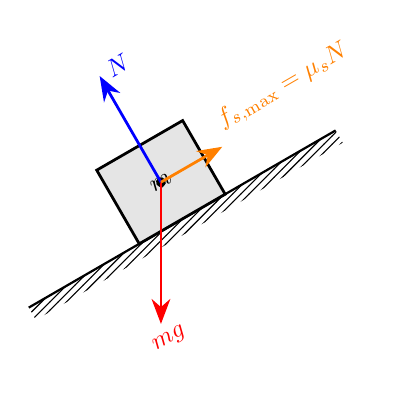
\begin{tikzpicture}[scale=0.9, transform shape, line width=1pt, rotate=30]
            % Ground (Incline)
            \draw[thick] (-2.5,0) -- (2.5,0);
            \fill[pattern=north east lines] (-2.5,-0.2) rectangle (2.5,0);
            
            % Mass
            \draw[fill=gray!20] (-0.7,0) rectangle (0.7,1.2);
            \node at (0, 0.6) {$m$};
            \fill (0, 0.6) circle (2pt);
            
            % Forces
            % Gravity goes straight down in world coords, not local. (Length = 2.0)
            \draw[-{Stealth[scale=1.2]}, red] (0, 0.6) -- ++(-120:2.0) node[below] {$mg$};
            % Normal Force (N = mg * cos(30) = 2.0 * 0.866 = 1.73)
            \draw[-{Stealth[scale=1.2]}, blue] (0, 0.6) -- ++(90:1.73) node[right] {$N$};
            
            % Friction pointing up the incline (f_s = mg * sin(30) = 2.0 * 0.5 = 1.0)
            \draw[-{Stealth[scale=1.2]}, orange] (0, 0.6) -- ++(0:1.0) node[above right] {$f_{s,\text{max}} = \mu_s N$};
            
            % Angle of incline indication (draw in regular coords if we want, but tricky in rotated env)
        \end{tikzpicture}
        
        \vspace{0.2cm}
        \small (b) On the verge of slipping down an incline
    \end{minipage}
    
    \caption{Free-Body Diagrams showing the variable nature of Static Friction.}
\end{figure}

\subsection{Kinetic (Dynamic) Friction ($\vec{f}_k$)}
Kinetic friction occurs when two surfaces \textbf{are slipping} or sliding past each other.
\begin{itemize}
    \item \textbf{Constant Force:} Unlike static friction, kinetic friction is generally considered constant regardless of how fast the object is sliding.
    \item \textbf{Formula:} 
    \begin{equation}
        f_k = \mu_k N
    \end{equation}
    where $\mu_k$ is the coefficient of kinetic friction.
    \item \textbf{Comparison:} For a given pair of surfaces, $\mu_k$ is almost always less than $\mu_s$ ($\mu_k < \mu_s$). It is harder to start moving a heavy box than it is to keep it moving!
\end{itemize}

\begin{figure}[h]
    \centering
    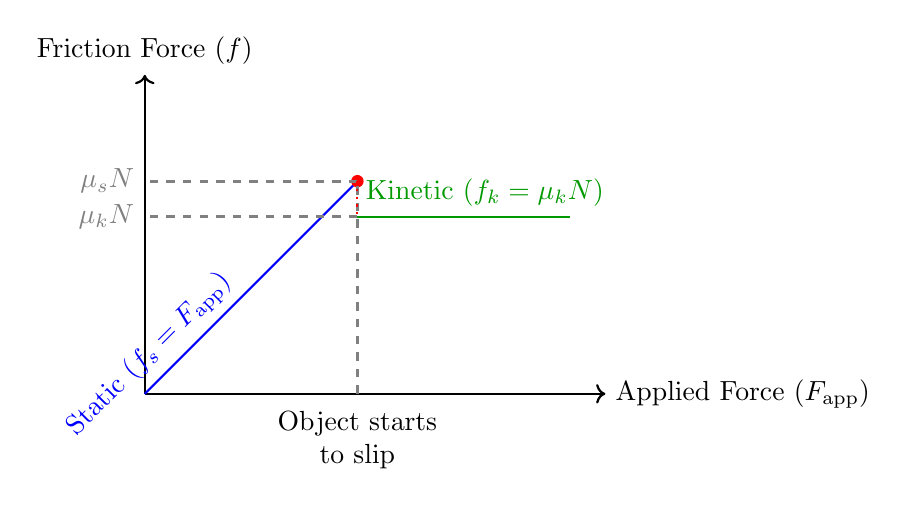
\begin{tikzpicture}[scale=0.9, line width=1pt]
        % Axes
        \draw[->, thick] (0,0) -- (6.5,0) node[right] {Applied Force ($F_{\text{app}}$)};
        \draw[->, thick] (0,0) -- (0,4.5) node[above] {Friction Force ($f$)};
        
        % Static region (y = x)
        \draw[thick, blue] (0,0) -- (3,3) node[midway, above left, rotate=45] {Static ($f_s = F_{\text{app}}$)};
        
        % Peak (max static)
        \fill[red] (3,3) circle (2.5pt);
        \draw[dashed, gray] (3,0) -- (3,3);
        
        % Kinetic region (constant y)
        \draw[thick, green!60!black] (3,2.5) -- (6,2.5) node[above, pos=0.6] {Kinetic ($f_k = \mu_k N$)};
        \draw[dashed, gray] (3,2.5) -- (0,2.5) node[left] {$\mu_k N$};
        \draw[dashed, gray] (3,3) -- (0,3) node[left] {$\mu_s N$};
        
        % Drop transition
        \draw[thick, dotted, red] (3,3) -- (3,2.5);
        
        % Labels on X axis
        \node[below, align=center] at (3,-0.1) {Object starts\\to slip};
    \end{tikzpicture}
    \caption{Friction Force versus Applied Force.}
\end{figure}

\newpage

\section{Free-Body Diagrams (FBD) and System Diagrams}

Before solving a problem, we often need to sketch forces. We use two types of diagrams depending on our approach:
\begin{itemize}
    \item \textbf{System Diagram:} A sketch that shows multiple objects treated together as a single ``system'' (e.g., two blocks connected by a string). Only \textbf{external forces} acting on the entire system are drawn. \textbf{Internal forces} (like the tension in the string connecting them) cancel out and are NOT drawn.
    \item \textbf{Free-Body Diagram (FBD):} A sketch that isolates \textbf{one single object}. You draw \textbf{all forces} acting on that specific object, including forces that were considered ``internal'' in the system view.
\end{itemize}

\subsection{Rules for Drawing Force Diagrams (Individual or System)}
The rules are exactly the same whether you are isolating a single object or grouping multiple objects into a system:
\begin{enumerate}
  \item \textbf{Define your boundary:} Choose exactly one object OR one well-defined system.
  \item Draw a single dot or box to represent your choice.
  \item Draw \textbf{only the external forces} crossing your boundary to act on that object/system.
  \item Label forces clearly ($N$, $T$, $mg$, $f$).
  \item Choose axes that simplify the math (e.g., align one axis with the direction of acceleration).
\end{enumerate}



\end{document}
